\documentclass{acm_proc_article-sp}
%\documentclass[final]{proceedings}

\usepackage{epsfig}
\usepackage{graphicx}
\usepackage{makeidx}
\usepackage{multicol}
%\usepackage{subeqn}
\usepackage{url}

%%%%%%%%%%%%
% material borrowed form nsf/linalg05 in futile attempt to define \newblock
%\documentclass[12pt]{article}
%\usepackage{nsf} %%% Erich's NSF proposal style (itr/nsf.sty)
%\usepackage{mathptm} %%% postscript times; does not screw up pdf formats
%\usepackage{newlfont}
%\usepackage{xspace}
%\usepackage{array}
%\usepackage{amsmath}
%\usepackage{amsfonts}
%\usepackage{longtable}
%\usepackage{rotating}
%%%%%%%%%%%%

%\usepackage{crop}
%\crop
%\makeindex

%\usepackage{natbib}
%\bibpunct[,]{[}{]}{,}{a}{}{,}

%%%%%%%%%%%%%%%%%%%%%%%%%%%%%%
% Libraries
%%%%%%%%%%%%%%%%%%%%%%%%%%%%%%

\newcommand{\lin}{Linbox }
\newcommand{\giv}{Givaro }
\newcommand{\aun}{Athapascan-1 }

%%%%%%%%%%%%%%%%%%%%%%%%%%%%%%
% Math character definitions:
%%%%%%%%%%%%%%%%%%%%%%%%%%%%%%


\def\N{\mbox{I\hspace{-.15em}N}}
%\def\Z{\mbox{Z\hspace{-.3em}Z}}
%\def\C{\mbox{C\hspace{-.6em}$\mid$}}
%\def\R{\mbox{I\hspace{-.15em}R}}
\def\K{\mbox{I\hspace{-.15em}K}}
\def\F{\mbox{I\hspace{-.15em}F}}
\def\bO{\mathcal O}
\def\Q{\mathbb Q}
\def\C{\mathbb C}
\def\Z{\mathbb Z}
\def\Io{\mbox{[\hspace{-.15em}[}}
\def\Ic{\mbox{]\hspace{-.15em}]}}
%\newcommand{\F}{{\mathsf F}}
%\newcommand{\C}{{\mathsf C}}
%\newcommand{\R}{{\mathsf R}}
%\newcommand{\K}{{\mathsf K}}
%\newcommand{\Z}{{\mathsf Z}}
\newcommand{\pints}{{{\mathsf Z}_(p)}}
\newcommand{\nxn}{{n\times n}}
\newcommand{\rxr}{{r\times r}}
\newcommand{\rxn}{{r\times n}}
\newcommand{\nx}[1]{{n\times #1}}
\newcommand{\rx}[1]{{r\times #1}}
\newcommand{\mx}[1]{{m\times #1}}
\newcommand{\zerobar}{{\bar 0}}
\newcommand{\bbar}{{\bar b}}
\newcommand{\fbar}{{\bar f}}
\newcommand{\rbar}{{\bar r}}
\newcommand{\ubar}{{\bar u}}
\newcommand{\vbar}{{\bar v}}
\newcommand{\wbar}{{\bar w}}
\newcommand{\xbar}{{\bar x}}
\newcommand{\ybar}{{\bar y}}
\newcommand{\calL}{{\mathcal L}}
\newcommand{\norm}[1]{{\|#1\|}}
\newcommand{\from}{~\mbox{from}~}
%\newcommand{\to}{~\mbox{to}~}
%\newcommand{\max}{~\mbox{max}~}
%\newcommand{\min}{~\mbox{min}~}

\newcommand{\range}[2]{{[#1,#2]}}
\newcommand{\irange}[2]{{[#1..#2]}}
%\newcommand{\irange}[2]{{\Io #1,#2 \Ic}}

\newcommand{\nats}{\ensuremath{\mathbb N}}
\newcommand{\ints}{\ensuremath{\mathbb Z}}
\newcommand{\reals}{\ensuremath{\mathbb R}}
\newcommand{\rats}{\ensuremath{\mathbb Q\mskip1mu}}
\newcommand{\cmplx}{\ensuremath{\mathbb C}}
\newcommand{\gf}{\ensuremath{\mathbb F}}

\newcommand{\bull}{{$\bullet$}}

\newcommand{\gfc}{{\overline{\mathbb F}}}
\newcommand{\setmid}{{\thinspace \mid \thinspace}}
\newcommand{\setsep}{{\thinspace : \thinspace}}

\newcommand{\softO}{{O\mskip1mu\tilde{\,}\mskip1mu}}
\newcommand{\til}{\lower 3pt\hbox{\large$\tilde{\ }$}}

\newcommand{\divs}{{\mskip3mu|\mskip3mu}}
\newcommand{\ndivs}{\nmid}

\newcommand{\trans}{t}

\newcommand{\floor}[1]{{\left\lfloor #1 \right\rfloor}}
\newcommand{\ceil}[1]{{\left\lceil #1 \right\rceil}}
\newcommand{\jac}[2]{{\binom{#1}{#2}_{\hbox{\tiny J}}}}
\newcommand{\vstrut}[1]{\rule{0pt}{#1}}
\newcommand{\hstrut}[1]{\rule{#1}{0pt}}
\newcommand{\nonzero}{{\setminus\{0\}}}
\newcommand{\iso}{\cong}

\newcommand{\longdash}{{\hspace{1.5pt}---\hspace}{1.5pt}\ignorespaces}

%\DeclareMathOperator{\GF}{GF}
%\DeclareMathOperator{\GL}{\textup{GL}}
%\DeclareMathOperator{\gal}{Gal}
%\DeclareMathOperator{\cont}{cont}
%\DeclareMathOperator{\disc}{disc}
%\DeclareMathOperator{\rank}{rank}
\newcommand{\rank}[1]{\ensuremath{\mbox{\tt rank}(#1)}}
%\DeclareMathOperator{\Span}{span}
%\DeclareMathOperator{\diag}{diag}
\newcommand{\diag}{\mbox{ diag}}
%\DeclareMathOperator{\Gcd}{gcd}
%\DeclareMathOperator{\sign}{sign}
\newcommand{\sign}{\mbox{ sign}}
%%\DeclareMathOperator{\rad}{Rad}
%\DeclareMathOperator{\Norm}{norm}
%\DeclareMathOperator{\adj}{adj}
%\DeclareMathOperator{\ord}{ord}
%\DeclareMathOperator{\Ord}{Ord}
%\DeclareMathOperator{\End}{End}
%\DeclareMathOperator{\prob}{Prob}
%\DeclareMathOperator{\rem}{rem}
%\DeclareMathOperator{\res}{Res}
%\DeclareMathOperator{\lcm}{lcm}
%\DeclareMathOperator{\divi}{div}
%\DeclareMathOperator{\li}{li}
%\DeclareMathOperator{\re}{Re}
%\DeclareMathOperator{\im}{Im}
%\DeclareMathOperator{\MM}{MM}
%\DeclareMathOperator{\M}{M}
%\DeclareMathOperator{\nequiv}{\mskip4mu\not\equiv\mskip4mu}
%\DeclareMathOperator{\nin}{\mskip4mu\not\in\mskip4mu}
%\DeclareMathOperator{\Tr}{Tr}
%\DeclareMathOperator{\Null}{Null}
%\DeclareMathOperator{\eqdef}{\overset{def}{=}}
%%\DeclareMathOperator{\charpoly}{\textup{char}}
%%\DeclareMathOperator{\minpoly}{\textup{min}}
%%\reDeclareMathOperator*{\charpoly}{\textup{charpoly}}
%\newcommand{\charpoly}{\textup{charpoly}}
%%\reDeclareMathOperator*{\minpoly}{\textup{minpoly}}
\newcommand{\charpoly}[1]{\ensuremath{\mbox{\tt charpoly}(#1)}}
\newcommand{\minpoly}[1]{\ensuremath{\mbox{\tt minpoly}(#1)}}
\newcommand{\shiftminpoly}[1]{\ensuremath{\mbox{\tt shiftminpoly}(#1)}}
%%\reDeclareMathOperator*{\valence}{\textup{valence}}
%%\reDeclareMathOperator*{\minvalence}{\textup{valence}}
%%\reDeclareMathOperator*{\charvalence}{\textup{characteristic valence}}
%\DeclareMathOperator{\charpoly}{\textup{charpoly}}
%\DeclareMathOperator{\minpoly}{\textup{minpoly}}
%\DeclareMathOperator{\valence}{\textup{valence}}
%\DeclareMathOperator{\minvalence}{\textup{valence}}
%\DeclareMathOperator{\charvalence}{\textup{characteristic valence}}

%%%%%%%%%%%%%%
% Matrices
%%%%%%%%%%%%%%
\newenvironment{jmatrix}{\left[\begin{array}{ccc}}{\end{array}\right]}
\newenvironment{smatrix}{\bigl[\begin{smallmatrix}}{\end{smallmatrix}\bigr]}

%%%%%%%%%%%%%%
% Algorithmes
%%%%%%%%%%%%%%
\newlength{\Stmtindent}
\makeatletter
\newenvironment{algorithm}[1]
{
   \setlength{\Stmtindent}{10pt}
   \def\Stmt{\@ifnextchar[{\@Stmt}{\@Stmt[]}}
   \def\@Stmt[##1]{\par\hspace*{\Stmtindent}\llap{##1\enspace\hfil}%
                   \hangindent\Stmtindent\ignorespaces}
   \def\Inspec{\par\hangindent0pt\noindent%
               \rlap{\@alginheader}\gdef\@alginheader{}%
               %\hspace*{1.0\Stmtindent}\llap{--\enspace}% was 4.5 (bds)
               \hangindent1.0\Stmtindent\ignorespaces}
   \def\Outspec{\par\hangindent0pt\noindent%
                \rlap{\@algoutheader}\gdef\@algoutheader{}%
                %\hspace*{1.0\Stmtindent}\llap{--\enspace}%
                \hangindent1.0\Stmtindent\ignorespaces}
   \def\Procspec{\par\hangindent0pt\noindent%
                \rlap{\@algprocheader}\gdef\@algprocheader{}%
               % %\hspace*{1.0\Stmtindent}\llap{--\enspace}%
                \hangindent1.0\Stmtindent\ignorespaces
				}
   \def\>{\advance\hangindent\Stmtindent\hspace*{\Stmtindent}\ignorespaces}
   \def\@alginheader{Input:}
   \def\@algoutheader{Output:}
   \def\@algprocheader{Method:}

   \parindent=0pt
   \parskip=1pt

   \medbreak\par {\bf Algorithm: }{\tt #1}
}
{\smallbreak}




%\newtheorem{lemma}[equation]{Lemma}
\newtheorem{conjecture}[equation]{Conjecture}
\newcommand{\R}{{\mathbb R}}
\renewcommand{\H}{{\mathcal H}}
\newcommand{\ch}[1]{#1^\vee}
\newcommand\brach[2]{\langle#1,\ch#2\rangle}
\newcommand{\Hom}{\text{Hom}}

\newcommand{\EE}{\ensuremath{{\mbox{E}8}~}}
\newcommand{\Prob}{\ensuremath{\mbox{Prob}}}
\newcommand{\QED}{\ensuremath{\Box}}
\newcommand{\alts}{\ensuremath{\mbox{ac}}}
\newcommand{\trace}{\ensuremath{\mbox{trace}}}
\newcommand{\coeff}{\ensuremath{\mbox{coeff}}}
\newcommand{\cra}{\ensuremath{\mbox{CRA}}}
%\newcommand{\signature}{\ensuremath{\mbox{S}}}
\newcommand{\reveal}{\ensuremath{\mbox{\tt reveal }}} 
\newcommand{\signature}{\ensuremath{\sigma}}
\newcommand{\lpm}{\ensuremath{\mbox{lpm}}}
\newcommand{\LUfailure}{\ensuremath{\mbox{LU\_failure}}}
\newcommand{\step}{\ensuremath{\mbox{step}}}
\newcommand{\abs}[1]{\ensuremath{|#1|}}
\newcommand{\prev}{\ensuremath{\mbox{prev\_sign}}}
\newcommand{\M}[2]{\ensuremath{J_{#2}({#1})}}
\newcommand{\p}{\ensuremath{p}}
\newcommand{\z}{\ensuremath{z}}
\newcommand{\n}{\ensuremath{n}}

% definitions used by included articles, reproduced here for 
% educational benefit, and to minimize alterations needed to be made
% in developing this sample file.

\newcommand{\pe}{\psi}
\def\d{\delta} 
\def\ds{\displaystyle} 
\def\e{{\epsilon}} 
\def\eb{\bar{\eta}}  
\def\enorm#1{\|#1\|_2} 
\def\Fp{F^\prime}  
\def\fishpack{{FISHPACK}} 
\def\fortran{{FORTRAN}} 
\def\gmres{{GMRES}} 
\def\gmresm{{\rm GMRES($m$)}} 
\def\Kc{{\cal K}} 
\def\norm#1{\|#1\|} 
\def\wb{{\bar w}} 
\def\zb{{\bar z}} 

% some definitions of bold math italics to make typing easier.
% They are used in the corollary.

\def\bfE{\mbox{\boldmath$E$}}
\def\bfG{\mbox{\boldmath$G$}}
\def\ZZ{\mbox{\boldmath$Z$}}
\def\P{\ensuremath{\mbox{\boldmath$P$}}}
\def\linbox{LinBox}
\def\nnz{\mbox{ nnz }}
\def\ord{\mbox{ ord}}
\def\order{\mbox{ dim}}
\def\for{\mbox{ for }}
\def\cond{\mbox{\boldmath$~|~$}}
\def\issym{\mbox{ is symmetric}}
\def\colamd{\mbox{ COLAMD }}

%\usepackage{latexsym}              % Additional LaTeX Symbols
%\usepackage{amssymb}               % AMS Fonts
%\usepackage{amsmath}               % AMSLaTeX
%\usepackage{amsthm}                % AMSLaTeX Theorem Environment

\newcommand{\Hadamard}{\mbox{the Hadamard bound}}
                                                                                
\newtheorem{definitions}{Definitions}
%\newtheorem{definition}{Definition}
\newtheorem{theorem}{Theorem}
%\newtheorem{notation}{Notation}
\newtheorem{notations}{Notations}
\newtheorem{proposition}{Proposition}
\newtheorem{corollary}{Corollary}
\newtheorem{lemma}{Lemma}

\newcommand{\pSize}{\ensuremath{\mathsf M}}
\newcommand{\rSize}{\ensuremath{\Omega}}
\def\normoo#1{\|#1\|_\infty} 
\newcommand{\set}{\ensuremath{\mathcal P}}
\newcommand{\minPrime}{\ensuremath{\beta}}
\newcommand{\length}{\ensuremath{\mathit l}}
\newcommand{\List}{\ensuremath{\mathcal L}}
\newcommand{\lcm}{\ensuremath{\mbox{lcm}}}


%\advance\topmargin by +0.2in

\begin{document}

%
% --- Author Metadata here ---
\conferenceinfo{ISSAC}{'05, KLMM, Chinese Academy of Sciences, Beijing, China}
%\setpagenumber{50}
%\CopyrightYear{2005} % Allows default copyright year (2002) to be over-ridden - IF NEED BE.
%\crdata{0-12345-67-8/90/01}  % Allows default copyright data (X-XXXXX-XX-X/XX/XX) to be over-ridden.
% --- End of Author Metadata ---

\title{Signature of Symmetric Rational Matrices and the Unitary Dual of Lie Groups
%\titlenote{A full version of this paper is available as ...
%
}
\subtitle{[Extended Abstract]}

% e-mail address. Additionally, tag each line of
% affiliation/address with \affaddr, and tag the
%% e-mail address with \email.
\numberofauthors{3}
\author{
\alignauthor Jeffrey Adams\titlenote
{Supported by NSF grant DMS 0200851.}\\
       \affaddr{Department of Mathematics}\\
       \affaddr{University of Maryland}\\
       \affaddr{College Park, MD, 20742 USA}\\
       \email{jda@math.umd.edu}
\alignauthor B. David Saunders\titlenote
{Supported by NSF grants CCR 0098284 and 0112807.}\\
       \affaddr{Department of Computer and Information Sciences}\\
       \affaddr{University of Delaware}\\
       \affaddr{Newark, DE, 19716 USA}\\
       \email{saunders@cis.udel.edu}
\alignauthor Zhendong Wan{\raisebox{9pt}{\dag}}
%\titlenote{Supported by NSF grants CCR 0098284 and 0112807.}\\
       \affaddr{Department of Computer and Information Sciences}\\
       \affaddr{University of Delaware}\\
       \affaddr{Newark, DE, 19716 USA}\\
       \email{wan@cis.udel.edu}
}
\date{14 January 2005}
\maketitle
\begin{abstract}
A key step in the computation of the unitary dual of a Lie group is
the determination if certain rational symmetric matrices are positive
semidefinite. The size of some of the computations dictates that high
performance integer matrix computations be used.  We explore the
feasibility of this approach by developing three algorithms for
integer symmetric matrix signature and studying their performance both
asymptotically and by experimenting on a particular matrix family
constructed from the exceptional Weyl group E8.  We conclude that the
computation is doable, with a parallel implementation needed for the
largest representations.
%A fundamental duality conjecture about group representations may be verified
%for some groups via a finite computation: determinations of positive definiteness
%of certain rational symmetric matrices.  The size of some of the computations dictates
%that high performance integer matrix computations be used.  We explore the feasibility
%of this approach by developing three algorithms for integer symmetric matrix signature 
%and studying their performance both asymptotically and by experiment on a particular matrix 
%family constructed from the exceptional Weyl group E8.
%We conclude that the computation is doable, with a parallel implementation needed
%for the largest representations.


\end{abstract}

% A category with the (minimum) three required fields
\category{G.4}{Mathematical Software}{Algorithm Design and Analysis}
%A category including the fourth, optional field follows...
%\category{J.2}{Physical Sciences and Engineering}[Mathematics]
\category{F.2.2}{Analysis of Algorithms and Problem Complexity}
{Nonnumerical Algorithms and Problems}[Computations on discrete structures]

\terms{Algorithms, Performance}

\keywords{
matrix signature, symmetric matrix, {L}ie group}
% NOT required for Proceedings

\section{Introduction}
%In the study of Lie group representations it is helpful to determine key
%properties of certain operators, which in the matrix representations are
%dense matrices with integer or rational number entries.  At issue is to compute
%which of these are positive definite, semi-definite or have other pattern of
%eigenvalue signs.

We propose, analyze, and test several algorithms for 
computing the signature and for verifying or disproving specific
definiteness properties of symmetric integer matrices.  
The latter is sometimes easier than the signature.  
Also there is often a considerable difference in the 
cost of verifying (certifying) a property and of certifying it's negation.
This is primarily an experimental paper whose purpose is to assess the feasibility 
of exact integer linear algebra methods for signature and definiteness determinations
that are useful in the study of Lie group representations.
The combination of measurements and analysis of asymptotic growth rates of time
and memory use that we provide is for the purpose of predicting the cost of the larger
computations of interest, so as to determine the most promising algorithms and the 
hardware resource needs.
The algorithmic asymptotic complexities reported here are largely straightforward 
applications of known results. 
We have an interesting observation which
allows both efficient binary tree structured Chinese remaindering to be used to construct 
numbers moduli a bunch of distinct primes and an early termination strategy at the same time.
Practical and asymptotic speed up is given when using early termination.
We have measured the time and memory costs of three algorithms on some matrices arising
in group representations, 
studied their relative merits, and developed formulas to predict the costs for large matrices.
We remark that the largest computation we've succeeded in doing with
a standard package such as Mathematica is for a matrix of dimension
400, whereas the largest needed is for dimension 7168  Our measurements 
indicate it will be feasible.

In section 2, the motivation for this work in the study of Lie group
representations is presented.  This application creates large problems
straining our limits of time and memory.
In section 3 we present the proposed algorithms and discuss their mathematical
basis and complexity.
Also included is some discussion
of unimplemented alternatives and of the space issues for large instances
of the problems. In section 4, we apply these algorithms to the matrices from 
Lie group representations.
Finally, in section 5, experimental results are reported
and, in section 6, conclusions are drawn on the state of these problems.

\section{Lie Group Representations and Unitary Duality}
%Subject: revised draft
%Date: Tue, 18 Jan 2005 22:03:38 -0500
%\documentclass[11pt]{amsart}
%\newtheorem{lemma}[equation]{Lemma}
%\newtheorem{conjecture}[equation]{Conjecture}
%\newcommand{\R}{{\mathbb R}}
%\renewcommand{\H}{{\mathcal H}}
%\newcommand{\ch}[1]{#1^\vee}
%\newcommand\brach[2]{\langle#1,\ch#2\rangle}
%\newcommand{\Hom}{\text{Hom}}
%
%\begin{document}
%
%\title{Chapter 2}
%\maketitle

We assume some familiarity with root systems and Weyl groups, for example see 
\cite{humphreys_coxeter}.
We begin with a formal construction.  Let $R$ be a root system with
Weyl group $W$. Thus $R$ is a finite subset of $V=\R^n$ satisfying
certain properties; in particular for each $\alpha\in R$
the reflection $s_\alpha\in \Hom(V,V)$ takes $R$ to itself.  By
definition $W$ acts on $V$. We may choose simple roots
$S=\{\alpha_1,\dots, \alpha_n\}$ so that $W$ is generated by
$\{s_i=s_{\alpha_i}\,|\,i=1,\dots,n\}$, with relations
$\text{order}(s_is_j)=m_{i,j}$ for certain $m_{i,j}\in\{2,3,4,6\}$.
For $\nu\in V$ define $\brach \nu\alpha=2(\nu,\alpha)/(\alpha,\alpha)$. 
Let $V^+$ be the set of $\nu\in V$ which are dominant (i.e.,
$\brach v{\alpha_i}\ge0$ ($1\le i\le n$)).

Fix a finite dimensional representation $(\rho,V_\rho)$ of $W$.
Thus $\rho:W\rightarrow GL(V_\rho)$ is a group
homomorphism. Fix an invariant Hermitian form $(,)_\rho$ on
$V_\rho$ (i.e., satisfying
$(v_1,v_2)_\rho=(\rho(w)v_1,\rho(w)v_2)_\rho$ 
for all $v_1,v_2\in
V_\rho, w\in W$). 
Choose a matrix $J_\rho$ so that $(v_1,v_2)_\rho=v_1J_\rho v_2^t$.


For $\alpha\in R$ and  $\nu\in V^+$ we define 

\begin{equation}
\label{A}
A_\rho(\alpha,\nu)=\frac{1+\brach\nu{\alpha}\rho(s_{\alpha})}{1+\brach\nu{\alpha}}
\in\Hom(V_\rho,V_\rho).
\end{equation}

Let $w_\ell$ be the longest element of $W$ and choose a reduced expression
$w_\ell=s_{i_N}s_{i_{N-1}}\dots s_{i_1}$
$(1\le j\le N,\,1\le i_j\le n)$.
Set $w_0=1$  and define
$w_j=s_{\alpha_{i_j}}s_{\alpha_{i_{j-1}}}\dots s_{\alpha_{i_1}}$
%Set $w_\ell=1$  and define
%$w_j=s_{i_j}s_{i_{j-1}}\dots s_{i_1}$
$(1\le j\le N)$.
For $\nu\in V$ define
%$$
\begin{equation}
A_\rho(\nu)=\prod_{j=1}^{n-1}A_\rho(\alpha_{i_j},w_{j-1}\nu)\in\Hom(V_\rho,V_\rho)
\end{equation}
%$$
%$$
\begin{equation}
\mbox{and }
J_\rho(\nu)=A_\rho(\nu)J_\rho.
\end{equation}
%$$

\begin{lemma}
\label{properties}
\begin{enumerate}
\item $A_\rho(\nu)$ is independent of the choice of reduced
expression for $w_\ell$,
\item $A_\rho(0)=Id$ and $A_\rho(\delta)=0$ (unless $\rho$ is
  trivial) where $\delta$ is one-half
  the sum of the positive roots,
\item $\lim_{\nu\rightarrow\infty}A_\rho(\nu)=\rho(w_\ell)$,
\item $A_\rho(\nu)$ is invertible unless $\brach\nu{\alpha_i}=1$ for
some $i$,
\item Assume $w_\ell\nu=-\nu$. Then $(A_\rho(\nu)v_1,v_2)_\rho=(v_1,A_\rho(\nu)v_2)_\rho$ for all
$v_1,v_2\in V$, and $J_\rho(\nu)$ is symmetric.
\end{enumerate}
\end{lemma}

For proofs of this and other statements in this section see
\cite{barbasch_spherical} and 
%\cite{atlas_papers}.
\url{http://atlas.math.umd.edu/papers}.

Let $\H$ be the affine Hecke algebra of $W$ \cite[Chapter 7]{humphreys_coxeter}.
Associated to $\nu$ is an irreducible spherical representation $\tau_{\nu}$.


\begin{lemma}
\label{tau}
The representation $\tau_\nu$ of $\H$ is unitary if and only if 
for every irreducible representation $\rho$ of $W$, the operator
$J_\rho(\nu)$ is positive semi--definite.
\end{lemma}

It is also of interest to determine the signature of $J_\rho(\nu)$.

The denominator in \eqref{A} is a convenient normalization, which
makes Lemma \ref{properties}(2) and (3) hold. 
Since
$\nu\in V^+$ it is positive and does not affect whether
$J_\rho(\nu)$ is positive semi--definite.

The question of whether $J_\rho(\nu)$ is positive
semi--definite only depends on whether $1-\brach\nu\alpha$ is
positive, negative, or $0$, for each $\alpha\in R$. Therefore the set
of dominant parameters $\nu$ is decomposed into a finite number of
facets, each one determined by an element of $\{+,0,-\}^n$ (not every
such n-tuple arises). 
The classification of the unitary representations $\tau_\nu$ of 
$\H$ is therefore reduced to a finite calculation.

Each facet contains an element $\nu$ with rational coordinates. It is
well known we may choose a basis of $V_\rho$ so that $\rho(w)$ is
a rational, or even an integral, matrix for all $w\in W$. For $n\le 8$
the former has been carried out explicitly in \cite{stembridge_models}, and
the latter in \cite{adams_models} except for $E_8$. Then the matrices
$A_\rho(\nu)$ and $J_\rho(\nu)$ will have rational
entries.  We may clear denominators when testing for positive
semi--definiteness. 

Now let $G$ be a split semisimple group over $\mathbb R$ or a $p$--adic
field $\mathbb F$, with root system
$R$.  Associated to $\nu$ is an irreducible spherical representation
$\pi_\nu$ of $G$.

\begin{lemma}
\label{padic}
If $\mathbb F$ is p--adic $\pi_\nu$ is unitary if and only if $\tau_\nu$ is unitary.
\end{lemma}

\begin{conjecture}
\label{conjecture}
If $\mathbb F=\mathbb R$ then $\pi_\nu$ is unitary if and only if
$\tau_\nu$ is unitary.
\end{conjecture}

Thus computing the unitary representations $\tau_\nu$ of Lemma
\ref{tau} tells us about a subset of the unitary dual of Lie groups
(the ``spherical'' unitary dual).

We may as well assume that $G$ is simple, or equivalently that $R$ is
irreducible. The irreducible root systems are of type
$A_n,B_n,C_n,D_n$ (classical) or $E_6,E_7,E_8, F_4$
or $G_2$ (exceptional).

The most interesting case is that of $E_8$.  The Weyl group has order
$696,729,600$; it has $112$ representations, the largest of which
has dimension $7,168$.  There are $1,070,716$ facets.

In the classical case the classification of the unitary
representations $\tau_\nu$, and Conjecture \ref{conjecture},
are known \cite{barbasch_spherical}.
Dan Barbasch and Dan Ciubotaru have also computed the unitary
$\tau_\nu$ in the exceptional cases.
Thus the problem which the calculation of $J_\rho(\nu)$ solves is
already known. However this calculation is the prototype of a much
more general calculation which will be needed to calculate the unitary
dual of Hecke algebras, real and $p$--adic Lie groups.

The Atlas of Lie Groups and Representations 
% \cite{lieatlas}
is a project to compute  the unitary dual by theoretical and computational
means, see \url{http://atlas.math.umd.edu}. 
Information about what computations are feasible is of
great importance in the continuation of this project.




%\bibliographystyle{plain}
%%\bibliography{/home/jda/tex/bibtex/master}
%\def\cprime{$'$} \def\cftil#1{\ifmmode\setbox7\hbox{$\accent"5E#1$}\else
%  \setbox7\hbox{\accent"5E#1}\penalty 10000\relax\fi\raise 1\ht7
%  \hbox{\lower1.15ex\hbox to 1\wd7{\hss\accent"7E\hss}}\penalty 10000
%  \hskip-1\wd7\penalty 10000\box7}
%\begin{thebibliography}{1}
%
%\bibitem{atlas_papers}
%Atlas of lie groups and representations: Papers.
%\newblock \tt atlas.math.umd.edu/papers.
%
%\bibitem{adams_models}
%J~Adams.
%\newblock Integral models of representations of weyl groups.
%\newblock \tt atlas.math.umd.edu/weyl/integral.
%
%\bibitem{barbasch_spherical}
%D.~Barbasch.
%\newblock Unitary spherical spectrum for split classical groups.
%\newblock preprint, {\tt www.math.cornell.edu/$\tilde{\ }$barbasch/nsph.ps}.
%
%\bibitem{humphreys_coxeter}
%James~E. Humphreys.
%\newblock {\em Reflection groups and {C}oxeter groups}, volume~29 of {\em
%  Cambridge Studies in Advanced Mathematics}.
%\newblock Cambridge University Press, Cambridge, 1990.
%
%\bibitem{stembridge_models}
%John~R. Stembridge.
%\newblock Explicit matrices for irreducible representations of {W}eyl groups.
%\newblock {\em Represent. Theory}, 8:267--289 (electronic), 2004.
%
%\end{thebibliography}
 % Jeff


\section{Signature Algorithms} %section 3

For the rest of this paper we will consider the question of signatures and
sign patterns
of symmetric matrices in general, but constantly keeping in mind the 
operators generated from Lie group matrix representations.
The signature of a real symmetric matrix $A$ is 
generally defined as $\sigma = \p - \n$, the number by which positive eigenvalues 
outnumber negative ones.  
%For our purposes, 
Define the {\em signature triple} to be the 
$\signature(A) = (\p, \z, \n)$, 
where $\p$ is the number of positive eigenvalues, $\z$ is the 
multiplicity of zero as an eigenvalue, and $\n$ is the number of negative eigenvalues.
A real symmetric matrix is 
positive definite if $z$ and $n$ are zero and 
positive semi-definite if $n$ is zero.

For a polynomial with only real roots, Descartes' rule of signs can be used to 
determine the number of positive roots and the number of negative roots.
Thus the signature triple of a matrix can be determined from the signs in 
the vector of coefficients of the characteristic polynomial.  
It is computationally useful that,
when only the zero eigenvalue has multiplicity greater
than 1, the characteristic polynomial is just a shift of the minimal 
polynomial.  If $A$ has minimal polynomial $m(x)$ of degree $d$, we define
the shifted minimal polynomial to be $x^{n-d} m(x)$.  
Less well known
is that signature can also be determined in certain cases, in a similar way, 
from the vector consisting of the leading principal minors of $A$. 
%We call such vectors $\signature$-revealing vectors for the matrix.
In view of these connections, for a vector the {\em signature triple} 
is 
$\signature(v) = (\p, \z, \n)$, where
$\p$ is the number of alternating successive nonzero pairs, and 
$\n$ is the number of constant successive nonzero pairs,
$\z$ is the number of zeros at the end of the vector
(which corresponds to the multiplicity of zero as an eigenvalue in our case).
To be precise, 
a pair of entries, $(v_i, v_j)$ of $(v_0, v_1, \ldots v_n)$ is {\em successive} 
if $i < j$ and the entries between them are zero.
A successive pair of nonzero entries is {\em alternating}({\em constant}) if 
their signs are opposite(same).
%write a degree $n$ polynomial (such as the characteristic polynomial of $A$)
%as $f(x)$ as $\sum_{i=0}^n f_i x^{n-i}$, with corresponding coefficient
%vector $(f_0, f_1, \ldots, f_n)$.
The vector in question will be either the coefficient vector of a polynomial or 
$w = (w_0 = 1, w_1, \ldots, w_n)$, where $w_i$ is $(-1)^i m_i$, with $m_i$ being
the $i\times i$ leading principal minor of the given matrix. 
Following \cite{KaLo96:issac},
say a matrix of rank $r$ has 
{\em generic rank profile} if the leading principal minors 
of dimensions 1 through $r$ are nonzero. 

\begin{theorem} [Signature theorem]{\label{theorem:sig}}
Let $A$ be a real symmetric $n\times n$ matrix.
The following hold:
\begin{enumerate}
\item 
Signature is invariant under congruence, that is, if 
$Q$ is nonsingular then $\signature(A) = \signature(QAQ^T)$.
\item
$\signature(A) = \signature(\charpoly{A})$.
Also, if the nonzero eigenvalues of $A$ are distinct,
$\signature(A) = \signature(\shiftminpoly{A})$.
\item
If $A$ is in generic rank profile with rank $r$, 
$$\signature(A) = \signature(1, -m_1, \ldots, (-1)^r m_r, 0, \ldots, 0),$$
where $m_i$ is the $i$th leading principal minor of $A$, and the last $(n-r)$
entries are zero.
\item
A matrix in generic rank profile has a unique $A = LDL^T$ decomposition with 
unit lower triangular $L$ and diagonal $D = \diag(d_1, \ldots, d_n)$.  If $A$
has generic rank profile and rank $r$, then (ending with $(n-r)$ zeroes)\\
$\signature(A) = 
\signature(1, -d_1, d_1 d_2, \ldots, (-1)^r\prod_{1 \leq i \leq r}d_i, 0, \ldots, 0)$. 
%\signature(0, \ldots, 0, (-1)^r\prod_{1 \leq i \leq r}d_i, \rdots, d_2 d_1, -d_1, 1)$. 
\end{enumerate}
\end{theorem}

Proof.  A good source for these fundamental facts is \cite{gantmacher}.
In particular the third statement is a theorem of Jacobi, \cite[Chapter X, \S 3, theorem 2]{gantmacher}.
The fourth item follows since $d_i = m_i/m_{i-1}$.
See \cite[Chapter 4]{GoLo96} for a good discussion of $LDL^T$ decomposition.
\QED

The generic rank profile condition assures that the $m_i$ consist of nonzero entries followed
by zeros with no intermingling of zero and nonzero values, and the same applies to the 
diagonal D of the $LDL^T$ decomposition.
Interestingly, again see \cite{gantmacher}, the 
signature can be recovered even when there are some scattered zeroes among the nonzero 
leading minors, hence something less than generic rank profile is needed.  
We will not pursue this point further. 

%Let us say that a vector $v$, such as the
%characteristic polynomial coefficients or
%leading principal minors with alternative signs,
%is a {\em \signature-revealing vector} for $A$ 
%if $\signature(A) = \signature(v)$.
In this paper, we are interested in computing the characteristic polynomial,
minimal polynomial and leading principal minors of an integer matrix, all
of them can be represented as a vector of integers. 

The algorithms we
propose all work by computing images of a signature revealing vector 
mod a series of primes
and constructing the integer vector via the Chinese Remainder Algorithm.
Depending on the algorithm, the vector may be the coefficients of the 
characteristic polynomial, coefficients of the shifted minimal polynomial,
or vector of leading principal minors.
In most of these cases there can be {\em bad primes}.  For instance 
there are primes $p$ for which the minimal polynomial of image mod $p$ of $A$ 
is not the image mod $p$ of the integer minimal polynomial of $A$.  This 
leads to a shifted minpoly mod $p$ that is not a true image of the integer
shifted minpoly. Similarly
a prime may divide many leading principal minors of A (and the rank may be
lower mod $p$ than the integer rank).  Note that in both of these cases
the segment of non-zero values computed mod $p$ is shorter than it should be.
In the interest of presenting the Chinese Remaindering issues in a generic
way, isolated from the specific signature revealing vector, we here
refer to a {\em likely-image} function, which given $A$ and $p$, returns
a vector which is likely to be the image mod $p$ of the desired integer vector
but may not be, and if not, will be shorter.
%??? example for fake image???
We call a prime $p$ {\em good} if $\reveal(A, p)$ returns the correct image,
otherwise $p$ is {\em bad}.  If $p$ is bad, always vector returned is too short.

%An integer answer such as characteristic polynomial and
%minimal polynomial of an integer matrix is often done by modular methods.
%It works as follows: first compute the answer mod many different primes, 
%then use the Chinese remainder algorithm to reconstruct the integer answer,
%or lift the answer to a power of a single prime, then reconstruct the answer
%by its $p$-adic representation.
%If a rational answer is desired,
% rational reconstruction can be used to reveal the answer at the final step.

The key feature of this generic Chinese remainder algorithm for such vectors 
is its early termination technique.
%This algorithm takes a $\reveal$ fuction as an input. 
%Given input matrix $A$ and prime $p$,
%the $v_p = \reveal(A, p)$ function tries to compute the
%image of the revealing vector mod $p$, and return it.
%And the length of the output vector indicates if the output vector is 
%a correct answer: if the length of $v_p$ is equal to the length of the image of
%image of the revealing vector mod $p$, then they must be equal, 
%otherwise, the output is not correct.

\begin{algorithm} {GenCRA}\\
$[$Chinese Remainder Algorithm with early termination] 
\Inspec
\begin{itemize}
\item
  $A$, a symmetric integer matrix.
\item
  $v_p = \reveal(A, p)$, a function as described above.
 % taking two inputs $A$, $p$, and 
 % returning, for good primes, the mod $p$ image of the vector to be revealed.
 % The length of the nonzero initial segment of $v_p$ indicates whether the prime is good or bad.
\item
  $\set$, a set of primes.
  %%with minimal prime $\minPrime$.
\item
  $\rSize$, the random sample size for the certificate.
%\item
%  $\length$, the length of output vector.
\end{itemize}
\Outspec\\
The revealed vector $v$ with integer coefficients. \\
%\Stmt[1.]
%$r := -1$, initially guess rank is $0$\\
\Stmt[1.]
Set list $\List := \emptyset$.  This will be a list of pairs: (good prime, imaged answer
 mod that prime).\\
Set $\length = 0$.

\Stmt[2.]
choose a random vector $x$ of length $n$ with
entries independently and uniformly chosen 
from $[0, \rSize - 1]$.\\
\Stmt[3.]
Uniformly and randomly remove a prime $p$ from $\set$.
%until $p$ is not used before. Mark $p$ used.\\
\Stmt[4.]
call $v_p = \reveal(A, p)$. 
If the length of $v_p$ is less than $\length$, [reject] goto statement 3.
If the length of $v_p$ is greater than $\length$, [restart] reset $\List := \{(p, v_p)\}$.
Otherwise, [continue] append pair ($p$, $v_p$) to $\List$.\\
\Stmt[5.]
Use Chinese remainder algorithm to construct 
the certificate $c^{(i)}$ where $i$ the size of $\List$, such that
$c^{(i)} = x \cdot v_{q} \pmod {q}$, for each pair $(q, v_q)$ in $\List$.\\
This construction can be done by combining the previous result $c^{(i-1)}$ 
with the current residue and modulus.
\Stmt[6.]
If $i = 1$ or $c^{(i)} \not= c^{(i-1)}$, then goto statement 3.\\
Otherwise the termination condition, $c^{(i)} = c^{(i-1)}$,
is met.
Return the vector $v$, which is
constructed from pairs in $\List$ by the Chinese remainder algorithm,
such that $v = v_q \pmod q$, for every pair ($q, v_q$) in $\List$.
This construction can be done by using a divide-and-conquer method. 
%Quit gathering images when the termination condition is met, and 
%The Termination condition may be 
%deterministic, namely modulus greater than Hadamard bound bound,
%in which case the overall algorithm is Las Vegas.
%The Termination condition may be 
%probabilistic, namely stop by Zhendongs trick (fixme - to be explained here),
%in which case the overall algorithm is Monte Carlo.
\end{algorithm}

Notes:
\begin{enumerate}
\item
%The Chinese remainder algorithm can be used to construct a number $a$ from
%its remainders $r_1, \ldots, r_n$ moduli a bunch of odd primes $p_1, \ldots, p_n$, respectively.
In order to capture negative numbers, 
we normalize the final number $a$, 
such that $a$ lies between $[-(m-1)/2, (m-1)/2]$, 
where $m$=$\prod_{1\leq i \leq n} p_i$.
\item
The early termination technique which may be used to reduce the practical run time
has been studied before -see e.g. \cite{Emiris98,Kaltofen02, Eberly03}.
Here, we use a different and more efficient termination technique.
At each step, only one integer called a ``certificate" is constructed 
at each prime, instead of the entire vector answer. This method has almost
the same probability as the porbability when the whole answer is constructed at each prime.  It allows the more efficient divide and conquer remaindering
to be done for the $n$ values in the answer while using the incremental
remaindering only for the certificate.
This technique can be easily adopted to other cases,
such as solving non-singular integer systems over the rationals.
\item
Additional independent certificates can be used to reduce the error probability,
since the error for each independent certificate is independent.
In our experiments, we've used two independent certificates.  
\end{enumerate}
\begin{theorem}
The algorithm above computes the revealed vector with error probability at most 
%On the condition that the length of output is correct,
%the probability that output $v$ is not correct
%is at most
\[\frac{2}{\rSize} +
\frac{\log^2_{\minPrime}(2\length \rSize B)}
{\pSize^\prime - \log_{\minPrime}(2\length \rSize B)},\]
where $B$ is the infinity norm of the correct answer,
$\pSize^\prime$ is the number of good primes in $\set$,
and $\minPrime$ is the minimal prime in $\set$.
\end{theorem}
%such that either \reveal($v_p, A, p$) returns false
%or $v_p$ has length of less than $\length$.

Note: For a typical problem, such as characteristic polynomial, 
or minimal polynomial, it is easy to choose a reasonable set of primes 
and random sample size
such that the error probability is tiny.  And runs are independent. If you
repeat the algorithm, you square the error probability.

PROOF:
Let $\alpha$ denote the correct answer and
$c$ denote $x \cdot \alpha$. 
We assume early termination condition meets when 
$c^{(n)}$ is equal to $c^{(n-1)}$, for some number $n$. 
If both $\abs {c} \geq \normoo {\alpha}$ and
$c = c^{(n)}$ are true, then the algorithm returns the correct answer.
This is true since the modulo which is the porduct of these primes in $\List$ is at least 
$2 \normoo {\alpha}$ under these hyothesis.

If $x$ is a random vector with entries 
independently and uniformly chosen from the integer set of $[0, \rSize-1]$,
then $\Prob (\abs{x \cdot \alpha}) < \normoo{\alpha})$
$\leq \frac{2}{\rSize}$.
This is true since
there is at least one entry of $\alpha$, whose absolute value is
equal to $\normoo{\alpha}$.
Without loss of generosity, we assume $\abs {\alpha_0}$ = $\normoo{\alpha}$.
Then for any $x_1, \ldots, x_{\length-1}$, then there is at most two integers $x_0$, 
such that $\abs{x \cdot \alpha} < \normoo{\alpha}$.

The probability analysis of $c \not= c^{(n)}$ 
on the condition that early termination condition $c^{(n)} = c^{(n-1)}$ meets,
is straightforward - see e.g. \cite[Theorem 1.]{Kaltofen02} for details.

So the total error probability is at most 
$\frac{2}{\rSize} +
\frac{\log^2_{\minPrime}(2\length \rSize B)}
{\pSize^\prime - \log_{\minPrime}(2\length \rSize B)}$.
%
%Claim 2: For an integer $m$, if a random prime $p$ is uniformly chosen 
%from a cardinality $k$ subset of $\set$, then
%$\Prob(p | m) \leq \frac{\log(\abs{m})}{\log(\minPrime)k}$.
%This claim is true since there is at most $\frac{\log(\abs{m})}{\log(\minPrime)}$
%primes which are members of $\set$ and also divide $m$.
%
%When the early termination first meets at $c^{(n)} = c^{(n-1)}$,
%let us look at the probability of $c \not= c^{(n)}$.
%We have $c^{(n)} = c^{(n-1)}$, that means $c - c^{(n-1)} = 0 \pmod{p_n}$,
%and moreover, $\normoo {c - c^{(n-1)}} \leq 2\normoo{c}
%\leq 2 \length \rSize B$.
%
%For any fixed $n$, if $c \not= c^{(n-1)}$ and 
%a good prime $p_n$ is randomly uniformly chosen from $\set$,
%then $\Prob (p_n~|~(c - c^{(n-1)}))
%\leq \frac{\log_2(2\length \rSize B)}{\log(\minPrime) 
%(\pSize - \pSize^\prime - n)}$. 
%If $n$ is larger than
%$\frac{\log(2 \length \rSize B)}{\log(\minPrime)}$, 
%then $v$ must be equal to $c$.
%Since the constructed $v = c \pmod m$, and 
%$m = \prod_{1 \leq i \leq n}p_i > 2\normoo{c}$, 
%
%So when the early termination condition meets,
%$\Prob (c \not= c_{i-1}) \leq 
%\frac{(\log(2\length \rSize)^2}{(\log(\minPrime))^2 
%%(\pSize - \pSize^\prime - {\log(2 \length \rSize B)}/{\log(\minPrime)})}$.
%
%If both $\normoo{c} \geq \normoo{\alpha}$ and $c = c_n$ are true, then
%$v$ must be equal to the correct answer.
%So the  probability of
%$v \not= \alpha$ is
%at most
%$\frac{1}{\rSize}+$
%$\frac{\log^2(2\length \rSize B)^2}
%{\log^2(\minPrime) 
%(\pSize - \pSize^\prime - {\log(2 \length \rSize B)}/{\log(\minPrime)})}$.
\QED


The following theorem gives additional flexibility in using the strategies
for signature computation made available by {\tt GenCRA}.
\begin{theorem} {\label{theorem:random}}
Let $A$ be an $n\times n$ real symmetric matrix and let S be a set of nonzero
integers of sufficient size that $\epsilon = n^2 \log(n)^2/\abs{S}$ is as small as
desired.
\begin{enumerate}
\item
Let $D$ be a diagonal matrix whose $n$ diagonal entries are chosen
uniformly at random from $S$, 
and let $B = DAD^T$.  Then $$\Prob(\shiftminpoly{B} = \charpoly{B} \geq 1 - \epsilon.$$
\item
Let $Q$ be a butterfly matrix whose $n \log (n)$ defining entries are chosen
uniformly at random from $S$, 
and let $B=QAQ^T$.
Then $$\Prob(B \mbox{ is in generic rank profile}) \geq 1 - \epsilon.$$
\end{enumerate}
\end{theorem}

Proof:  These preconditionings are discussed in detail in \cite{CEKSTV02} \QED

For the generic rank profile condition, The butterfly is chosen as preconditioner
because the specified matrix $QAQ^T$ can be computed in $\softO(n^2)$ time.  
For our purposes here we can afford preconditioning complexity up to $\softO(n^3)$ time.
A general random matrix could be used for the preconditioner, or Toeplitz \cite{KS91} or sparse
preconditioners \cite[Section 6]{CEKSTV02}.
It is of interest to keep the size of the entries of the resulting matrix as small as
possible.

We build three algorithms on the theory described above, two using the minimal polynomial (for blackbox
and for dense matrices) and one using $LDL^T$ decomposition.

\begin{algorithm} {BBSM [BlackBox Signature by Minpoly]\label{bbsm}}
\\Input:  $A$, a symmetric matrix in blackbox form,\\
$S$, a set of integers from which to make random selections.
\\Output: The signature $\signature(A) = (p, z, n)$.
\Stmt[1.] $[$ Preconditioning may be necessary $]$
Let $q$ be a random prime.\\ 
Let $r := \rank{A,q}$ and $m_q = \minpoly{A, q}$.\\ 
%$[$ \rank{} and \minpoly{} can work even if $A$ is a rational matrix, 
%provided $q$ does not divide any denominator of $A$.$]$\\
If $\deg(m_q) < n \mbox{ and } \deg(m_q) \leq r$, 
let $B := DAD$ [A blackbox],
for a random diagonal matrix $D$ with entries chosen 
from $S$,\\
Otherwise, let $B := A$.\\
$[$ Now $B$ has the same signature as $A$ and its charpoly is 
its shifted minpoly, with high probability. ]
\Stmt[2.] Choose a set $\set$ of primes, and the sample size $\rSize$, such that
the error probability is as small as desired.
Return \signature($x^{\max(0, n-r-1)}$GenCRA$(B, \minpoly{}, \set, \rSize)$).

\end{algorithm} 

The $r = \rank{A, p}$ and $v = \minpoly{A, p}$ algorithms 
used to compute the rank and the minimal polynomial 
of $A$ mod $p$ respectively
are as in \cite{Wie86, KS91, CEKSTV02}, for example.  
Here \minpoly{} and \rank{} run in time $\softO(nE)$
and are probabilistic with probability
of error no more than $1/p$,
where $E$ is the cost of a single matrix-by-vector product.
But \rank{} will never return a value
greater than the true rank and \minpoly{} always computes at least a factor
of the true minimal polynomial of $A$ mod $p$. 
%It will returns true or false dependent on the degree of the minimal polynomial.
%(This is in addition to the possibility of a bad prime $p$.) 
%minpoly).  In any case the shift, \shiftminpoly{}, meets the requirements of {\tt image} for GenCRA.
$DAD$ is the blackbox whose matrix-vector product is formed as $y = D(A(Dx))$.
%Optimalization may be done for $DAD$.
%However, if $A$ itself is represented as an unexpanded product of sparse matrices, as in 
%\M{\nu}{\sigma},
%some time can be saved by explicit multiplication of $D$ into the first and last factors. 

\begin{algorithm} {DSM [Dense Signature by Minpoly] \label{dsm}}
\\Input: Matrix $A$, in dense form.
\\Output: $\signature(A)$.
\Procspec \\
Apply algorithm {\tt BBSM}, except use 
$r = \rank{A, p}$ \cite{DumasGiorgiPernet:2004:issac} and 
\\$v = \minpoly{B, p}$, \cite{Pernet03}, % wan pernet
algorithms which
are 
available for the explicit (dense) matrix representation.
Then $\rank{}$ and $\minpoly{}$ are deterministic eliminations running in time $\softO(n^3)$
and using O($n^2 d$) memory 
Of course, in this case the DAD preconditioning is done 
explicitly (and cheaply).
Again, of course, $p$ may be a bad prime (minpoly of A mod p not equal mod p 
image of integer minpoly of A.. 
\end{algorithm} 

Especially for blackbox matrices, it is useful that minpoly computation can suffice,
because we have faster algorithms for minpoly than for charpoly in that case.
But for the DSM algorithm above, an alternative is to use the charpoly() function as the $\reveal$ function, see \cite{Pernet03} for example.
% also cite keller-gehrig?
Also note that the minpoly suffices for determining the sign pattern (not full signature)
even without preconditioning.  
%To be precise, the sign pattern of $A$ is determined from 
%$s = \signature(\mbox{minpoly of A})$ 
%by replacing positive entries in $s$ by $+$, though the point is that
%the pattern may sometimes be more easily determined than the signature itself.
%In particular, 
When the minpoly is of low degree or has small coefficients, this is a great savings.
In general, though, BBSM is not a fully memory efficient algorithm because of the size of the 
\signature-revealing vector.  It is possible that the technique of \cite{BEPP97} could
be used to determine the signs using less memory and perhaps less time.  This approach
deserves further examination.

%However,
%it is not necessary to compute the characteristic or minimal 
%polynomial to answer signature and definiteness questions.  
Alternatively, 
combining Theorem \ref{theorem:sig}, part 3, 4, 
and theorem \ref{theorem:random},
part 2,  we may work from 
the $LDL^T$ decomposition of a matrix in generic rank profile.  
If the matrix should fail to have generic rank profile, this will be detected during
the eliminations because of the need for pivoting.
We use preconditioners $Q$ to assure that $QAQ^T$ has generic
rank profile.
In some cases symmetric pivoting could be used instead to avoid the 
increased entry size caused by preconditioning.  

The $LDL^T$ decomposition based signature algorithm assumes a procedure 
$\lpm(v, A, p)$ which 
computes the vector 
%$$((-i)^k\prod_{1\leq i \leq k}D_{i,i}, \cdots, D_{1,1}D_{2,2}, -D_{1,1}, 1),$$
%$$(1, -d_1, d_1 d_2, \ldots, (-1)^r\prod_{1 \leq i \leq k}d_i)$$ 
of leading principal minors with alternating signs as described above, 
up to but not including the first which is zero mod $p$.  
The matrix mod $p$ can fail to have generic rank profile.
We could modify the $LDL^T$ to successfully handle such cases, but it is a 
remote possibility and not worth the overhead.  
We simply reject such primes as bad primes.
The procedure $\lpm$ 
meets the requirements of a \signature-revealing function for GenCRA.  

\begin{algorithm}{DSLU}\label{siglu}\\
$[$Dense matrix Signature by LU-decomposition]\\
Input: $A$, an integer symmetric $k\times k$ matrix.\\
Output: Signature $\signature(A) = (\p, \z, \n)$.
\Stmt[1.] $[$ Preconditioning may be necessary $]$\\
Let $q$ be a random prime.\\ 
Let $\lpm(v_q, A,q)$, $r := \rank{A, q}$.\\
%$[$ \lpm can work even if $A$ is a rational matrix, 
%provided $q$ does not divide any denominator of $A$.$]$\\
If length of $v_q$ less than $r + 1$, let $B := QAQ^T$,\\
$~~~$ for a random integer matrix $Q$ with entries chosen\\ 
$~~~$ from $[1, \cdots, s]$ (or any set of $s$ nonzero integers).\\
$~~~$ [Q may be a Toeplitz or Butterfly matrix for speed]\\
Otherwise, let $B := A$.\\
$[$ Now B has the same signature as A and has generic rank profile. ]\\
Choose a set $\set$ of primes, and the sample size $\rSize$, such that
the error probability is as small as desired.
\Stmt[2.] %%$[$ Lift $]$\\
Return \signature($x^{n-r}$GenCRA$(B, \lpm(), \set, \rSize)$).
\end{algorithm}
%Cholesky mod primes?
\begin{theorem}
Let $A$ be an integer blackbox $\n \times n$ symmetric matrix,
whose matrix-vector product costs $e$ operations and 
whose entries would be of bit length at most $d$ if they were explicitly constructed.

Algorithms BBSM, DSM, and DSLU are Las Vegas probabilistic algorithm 
if the Hadamard bound is used and are
Monte Carlo if early termination is used in the remaindering.
Even with early termination, DSM is Las Vegas if the computed 
integer minimal polynomial is checked by evaluation at $A$ over the integers. 
This costs $\softO(n^4)$.% Zhendong check it.
Also a minimal polynomial verification by application to the identity 
could be done after
BBSM making it Las Vegas for the sign pattern of the signature.

Let $h$ be a bound for the bit lengths of the values constructed using GenCRA, 
(the length of the largest characteristic polynomial coefficient or of the 
largest leading principal minor).  Then the expected run times are in 
$\softO(neh)$ for BBSM and in $\softO(n^3h)$  for DSM and DSLU.
By the Hadamard bound, $h$ is in $\softO(nd)$, so the expected run times
are also in $\softO(n^2 e d)$ for BBSM and in 
$\softO(n^4d)$ for DSM and DSLU.

In particular if $e \in \softO(n)$, and $d \in \bO(\log(n))$,
then the BBSM expected run time is $\softO(n^3)$ and the DSM, DSLU expected times are in $\softO(n^4)$.
\QED
\end{theorem}

Also, with any of the \signature-revealing vectors, the entries tend to grow 
in proportion to their index.  In particular the $i$th entry is either an $i\times i$
minor or sum of $i\times i$ minors, so is bounded by the Hadamard bound which is in $\softO(id)$.
A heuristic to determine indefiniteness 
computes the first few vector entries, using many fewer remaindering steps than are required
for the later entries.  If the sign pattern fails to be constant or strictly alternating
the matrix is indefinite.  It is an open question whether a conjugacy class preconditioning,
$A \rightarrow QAQ^T$, could make probable that early entries indicate definiteness (cheaply).

\section {Application to Lie matrices}
The matrices from Lie group representation are rational matrices.
Our algorithms in the previous section focus on integer matrices.
There are at least two ways to adapt.
One is to compute the minimal polynomial, or the leading principal minors
over the rationals.
Rational numbers must be reconstructed at the GenCRA,
and it is easy to adopt our GenCRA, including the early termination technique,
to this case.
The other way is to multiply the matrices by the $\lcm$ of
the denominators of all entries.
For these specially constructed matrices from Lie group representation, 
the $\lcm$ of the denominators of all entries
is just a little larger than each individual one,
so this latter way is a better.
We found for some models that the $\gcd$ of all the
numerators in the dense representation is not trivial and  can be removed.

Next we present blackbox algorithms to compute the
$\lcm$ of denominators of all entries, 
and $\gcd$ of numerators of all entries,
respectively.
\begin{algorithm} {LD [LCM of Denominators]}
\Inspec \\
$A$, a rational matrix\\
$M$, sample size\\
$n$, number of trials
\Outspec \\
$d$, the $\lcm$ of denominators of all entries of dense representation of $A$.
\Stmt[1.]
for $i$ from $1$ to $n$ do\\
Choose a random vector $x^{(i)}$ with entries independently and uniformly chosen
from $[0, M-1]$\\
$y^{(i)} = A x^{(i)}$, apply $x^{(i)}$ to $A$\\
$d^{(i)}$= the $\lcm$ of denominators of every entry of $y^{(i)}$.
\Stmt[2.]
$d := \lcm (d^{(1)}, \cdots, d^{(i)})$
\Stmt[3.]
return $d$.
\end{algorithm}

\begin{algorithm}{GN [Gcd of Numerators]}
%\Inspec \\
%$A$, an integer matrix\\
%$M$, sample size\\
%$n$, number of trials
%\Outspec \\
%$g$, the $\gcd$ of all entries of dense representation of $A$.
%\Procspec\\
\\Apply algorithm {\em LD} by replacing $\lcm$ with $\gcd$ and 
denominators with numerators.
\end{algorithm}

The algorithm {\em LD}
always returns a factor of the true answer.
The algorithm {\em GN}
always returns a multiple of the true answer.
For a rational matrix $A$, if 
$d$ and $g$ are the $\lcm$ of all denominators 
and $\gcd$ all numerators of entries of $A$, respectively,
then If $A^\prime = \frac{d}{g}A$ is an integer matrix.
For each individual trial,
if all entries of  $A^\prime x^{(i)}$ are coprime,
then $d^{(i)}$ is correct in both algorithms.
Please see \cite{Saunders::LA::2004} for probability analysis. 
The error probability is roughly $2^{-n + 1}$.

Each matrix $J_\rho(\nu)$ in equation 3 can be represented as
a product of many sums of sparse matrices and scalar matrices.
%%$[\prod \frac1{r_i}(r_iT_i +I)]J_\rho$, where $T_i=\rho(s_{\alpha_i})$
%as in Section 2.
%%, and $T_i$ and $J_\rho$ are sparse matrices.
The algorithm BBSM is very suitable for this case.
We also reduce the product of $121$ sums of sparse matrices and scalar matrices
to a product of $94$ sparse matrices for the $E_8$ case. 
We explicitly compute each sum of a sparse matrix and a scalar matrix and 
store them as a single sparse matrix.  Also, if the result is a diagonal matrix,
explicitly multiply it into the previous factor.
By reducing the number of sparse matrices in this way, 
$20\%$ run time was saved for the BBSM algorithm. 
After multiplying these collapsed matrices 
by the $\lcm$ of denominators of all entries and dividing
by $\gcd$ of numerators, these matrices can be handled by the
algorithms discussed in the previous section.



%\section{Checking the Model and Operator}

\section{Experiments} %section 5
Our goal is to know which algorithm to use and how much resources it will take 
for computing the signature of %the $\M{\nu}{n} = \M{\nu}{\rho}$, 
the $\M{\nu}{\rho}$ in equation 3,
the matrix generated by the facet $\nu$
for the model of dimension $n$ of the group \EE.  
In particular, we focus on the case when
the facet is the challenge facet $\nu_0 = 1/40 (0,1,2,3,4,5,6,23)$, 
and the goal is to verify (or disprove) that $\M{\nu_0}{n}$ is positive definite.  
To emphasize the model dimension $n$ in what follows, let $J_n = \M{\nu_0}{\rho}$.

The three signature algorithms we have discussed are BBSM, DSM, DSLU.
We have computed full solutions by each model for the models
Q2, $\ldots$, Q12, Q22, Q32, Q42, Q52(dimension 1008),
and we have computed single modular step costs for every 10th model on up to the largest,
Q112(dimension 7168).
The experiments involved individual run times up to about one day and 
verified, where the full computation was done, that $J_n$ is indeed positive definite.
All computations reported here were performed on a 3.2GHz Xeon processor with 6GB of main memory.
%and xx L2 cache.
Our purpose here is to determine the algorithm to use and resources needed for the full 
signature computation on examples of all dimensions (up to 7168) and to have tools to 
estimate the cost for matrices defined by other facets.

The blackbox representation of $J_n$ is a product of very sparse factors. 
%Since the cost of computing the characteristic polynomial depends on 
%the cost of applying $A$ to a vector, 
%we examined the number of nonzero elements in total in these factors.
Since the blackbox method cost is sensitive to $e$, the cost of the single matrix-by-vector product, 
we examined the number of nonzero elements in total in these factors.
To guess the expected growth of $e$ with dimension, we measured the total number
of nonzero entries in the factors of every 10th model up to Q112.
Since the number of factors is fixed and they are extremely sparse we expect a linear or 
$n\log(n)$ term to dominate.  The formula 
$e = 132.5900691 n + 13.12471811 n \ln(n)$, a least squares fit to the data, is 
plotted in figure 1 along with the data values. 
The fit is extremely
good and we see that $e$ is only slightly super-linear.  Therefore we expect
the runtime of characteristic polynomial computation mod a single prime to grow at 
a rate only slightly above quadratic in $n$.
\begin{figure}[h] %1
\caption{Blackbox number of non-zeroes}
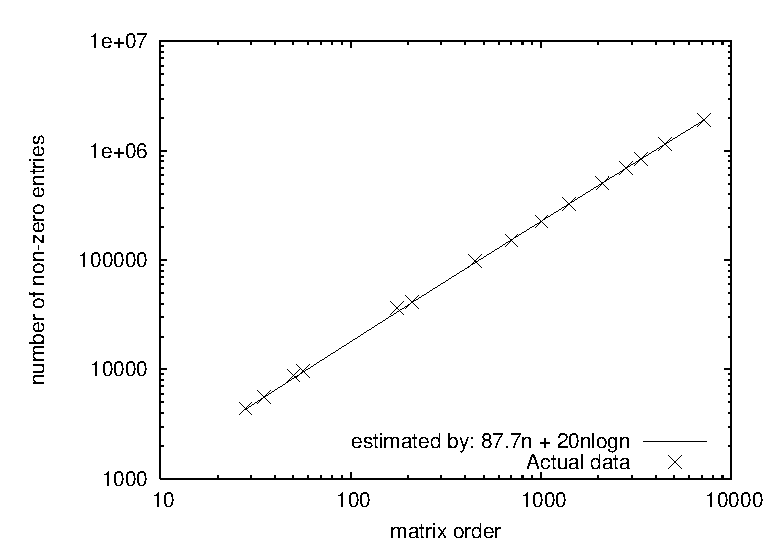
\epsfig{file=../graph/nonzero.eps,  
height=1.4in, width=.45\textwidth}  
\end{figure}

Each algorithm involves a series of steps mod primes $p_i$, each step being
a computation of \signature-revealing vector (a minpoly or diagonal of $LDL^T$-decomposition) 
mod $p_i$.
The computation is finished when the CRA remaindering has given an image of the vector
with modulus, \(M = 2 \prod p_i\), sufficiently large to recover the actual (signed) 
vector entries.  If we know a bound $d$ for the length of the entries of $J_n$,
we have by the Hadamard bound a maximal length $b = n(\log(n)/2 + d) + 1$ for $M$.

The dense matrices are computed by applying the black box to the columns of the 
identity matrix (over $\Z$, not modularly), and so the computation is 
sensitive to the length of the 
actual integer entries.
%of the expanded (and dense) matrix.
Let $d$ be the bit length of the 
largest entry.  
We do not have a theory to predict how matrix entry bit length $d$ may depend on the 
model dimension for a fixed facet. 
We have plotted the bit length $d$ of the largest entry of $J_n$ along with
the fitted curve $d = 67.7 + 33.2\log(n)$ in figure 2.  
One sees the $\log(n)$ playing a stronger role than that for the non-zeroes in the blackbox,
but the fit to the data is poorer and likely to have less predictive value.
We noted that the $n^2$ entries of $A$ all have about the same length, so $n^2 d$ accurately
describes the storage required for $A$.
\begin{figure}[h] %2
\caption{Bit length of entries}
%Dense matrix bits per entry}
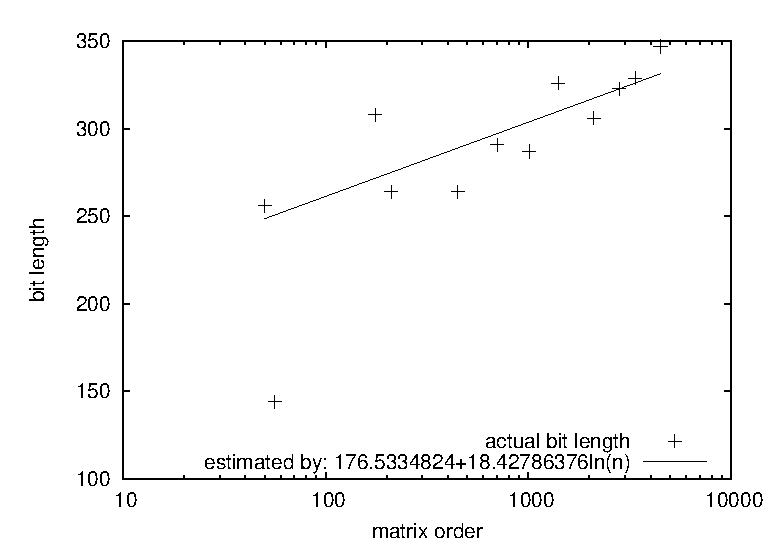
\epsfig{file=../graph/bits.eps, 
height=1.4in, width=.45\textwidth}  
\end{figure}

It will also be useful to use $d$ in estimating the number of remaindering steps.
The needed bit length $b$ for the modulus $M$ is at most 1 bit (for sign) more 
than the length of the Hadamard bound.  The rows norms are no more than \(\sqrt{n(e^d)^2}\),
so their product has length bounded by $n(\log(n)/2 + d)$.
Reasonably consistent with this prediction is the number of bits used when we ran
the full algorithms on $J_n$ for $n$ up to 1008 (model Q52).  
The curve in figure 3 is a least squares fit,
$b = 150.1 n + 17.30n ln(n)$,
The number of bits for the charpoly coefficients (sums of minors) are expected 
to be slightly larger than for the entries of the  leading principal minors vector,
but most likely, the final term, determinant of $J_n$, is dominant.  
The number of bits needed appears to be slightly super-linear, not quite as large as
the worst case Hadamard bound level.  
\begin{figure}[h] %3
\caption{Bit length of final modulus}
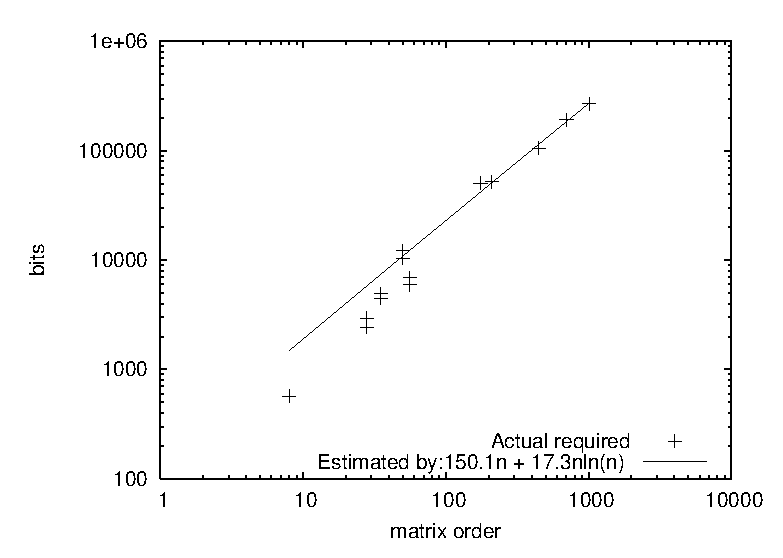
\epsfig{file=../graph/bit_required.eps, 
height=1.4in, width=.45\textwidth}  
\end{figure}

Next we consider the costs of the modular steps.
Let \step(s) denote the cost per step which varies with length, $s$, of the prime, 
but is essentially constant among primes of the same length.
The total time  is $b/s \times \step(s)$ when using $s$ bit primes. 
Thus we see the advantage of minimizing $\step(s)/s$, the cost per bit.
After discussing $\step(s)/s$ and determining it's value, for each algorithm,  
we will know how to estimate the full runtime of the algorithms.

We expect to be able to reduce the LU step cost
by half, as an elimination better tailored to symmetric matrices can be done, while still taking
advantage of block operations using BLAS. For the blackbox algorithm, block methods may 
be able to reduce the costs somewhat, and the DSM may perform relatively better than
here if the dense \charpoly{} algorithm \cite{Pernet03} % the KG based idea
is used rather than preconditioning.
At any rate, in figure 4 we see the performance of the modular steps of the three algorithms,
BBSM, DAME, DSLU as currently implemented.
Asymptotically, the BBSM step runtime, $s$, is expected to grow in
proportion to $ne$. There was a good fit to $s = 61 n^2\log(n)$ nanoseconds per bit
(recall that $e$ has a $n\log(n)$ dominant term).
The algorithms DSM and DSLU depend on the construction of the full integer matrix of 
$J_n$, which is done once.  The step times consist of computing a modular
image of that and proceeding with an elimination on the image.
The implementation of the Krylov matrix construction in the \minpoly{} algorithm of $DSM$,
uses a technique of recursive doubling to better exploit fast matrix multiplication,
and gets a step time $s$ which fits the formula 
$t = 1.8   n^3  + 0.16  n^3 \log(n)$ nanoseconds per bit.
$t = 0.37 n^3 \log(n)$ nanoseconds per bit.
quite well.  
The DSLU step fits 
$t = 0.3838888362 n^3$ nanosec/bit.
But these formulas have to be worked to the bit cost level!!!

The log factor for DSM step can be removed, so it remains possible that it can become 
competitive or participate with BBSM in a heterogeneous distributed computation, running
on the machines with larger memory.  
The time formula for the dense matrices should remain valid as long as the modular
step fits in main memory. After than swapping would dramatically increase times.
Assuming a memory capable of holding a 2GB virtual memory,
this would allow for $n^2$ words, so $n < 2^{15}$.  For all practical purposes,
the blackbox step has no memory limitation.
\begin{figure}[h]
\caption{Time per bit of modulus}
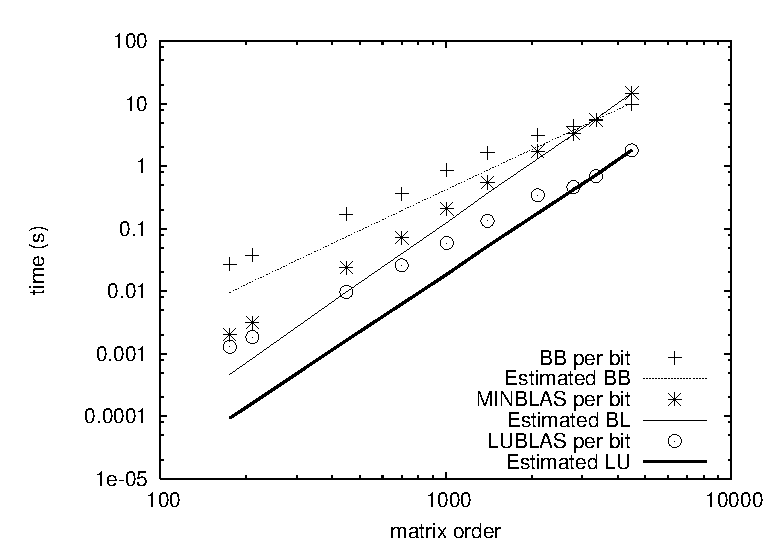
\epsfig{file=../graph/steps.eps,
height=1.4in, width=.45\textwidth}  
\end{figure}


The total runtime then involves the time per bit in the modular steps times the number
of bits in the \signature-revealing vector.  The Chinese remaindering adds a cost that
is similar for each but large enough to mute somewhat the effect of the differing step costs.
However with the early termination technique of the previous section this remaindering
is a smaller factor than in earlier timings.  
%For instance, without the asymptotic 
%improvement in the termination strategy our time for x was y, now it is z.
The two dense algorithms also incur a lower order
cost for the creation of the expanded integer matrix initially.
In figure 5 we show the overall run times (where the computations have been
done so far) together with their least squares fit formulas.
The formulas for time $t$ in nanoseconds are 
BBSM: $t = 10050 n^3 \log(n)$, % blackbox full time formula
DSM: $t = 6.08 n^4 \log(n)$, % blas full time formula
and DSLU: $t = 1.45 n^4 \log(n)$.% lu full time
%$t = 2240000 n^2  + 66800 n^3$ % blackbox full time formula
%$t = 12900 n^3  + 28.9 n^4$ % blas full time formula
%$t = 9650 n^3  + 0.222 n^4$ % lu full time
Theory predicts a second log factor in the BBSM time, coming from the 
the single matrix-by-vector product cost, $e$.
However that effect is weak and the fit was poorer.
\begin{figure}[h]
\caption{Total run time}
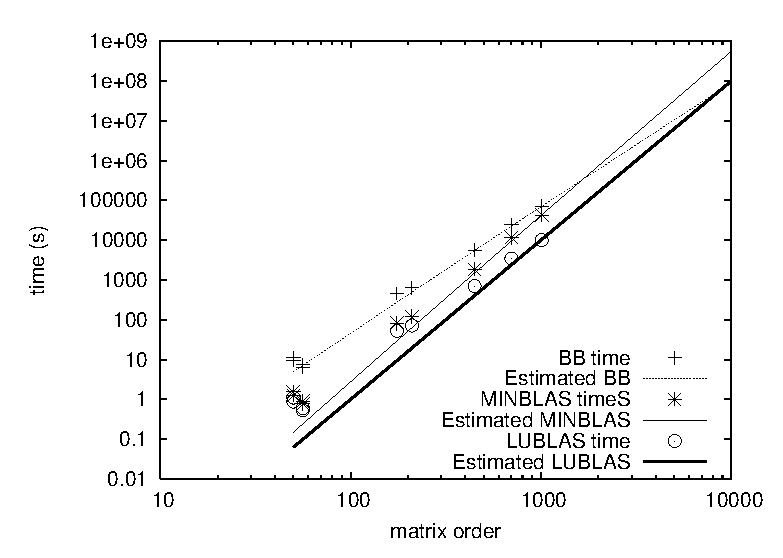
\epsfig{file=../graph/time.eps,
height=1.4in, width=.45\textwidth}  
\end{figure}

The memory needed to store the \signature-revealing vector mutes the memory 
advantage of BBSM.  However the modular images of the vector are easily stored on hard disk
and manipulated from there, so the memory advantage remains real.
The crossover point of the runtime formulas for BBSM and DSLU is around $n = 6931$. 
However the formula $t = 10.02 n^4$ fits the DSLU data about as well as our formula 
above.  Using that form, the crossover point is at $n = 9150$.

%$t = 0.002240174633 n^2  + 0.00006676817979 n^3$ % blackbox full time formula
%$t = 0.00001285796899 n^3  + 0.2885270500 10^{-7} n^4$ % blas full time formula
%$t = 0.9645194584 10^{-5}   n^3  + 0.2217193167 10^{-9}   n^4$ % lu full time

%\begin{figure}
%\caption{predict}
%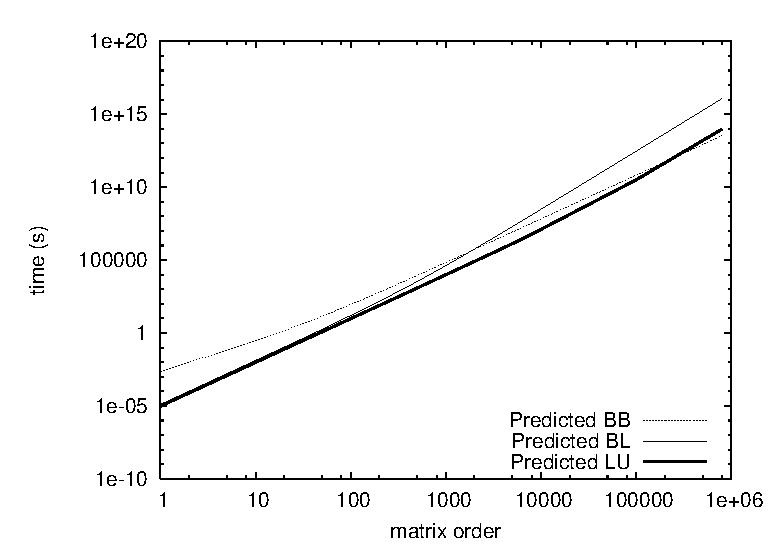
\epsfig{file=../graph/predict.eps,
%height=1.2in, width=.45\textwidth}  
%\end{figure}


%Optimizing prime length

%floating point and other things tried that were not much help.
%fixme talk floating point in alg section

%We have also completed a study of the operators for the facet
$1/12 (0,2,2,3,4,5,7,23)$.  In this case the ranks of the operators in
each model are very low.
For the largest model of dimension 7168 the rank is 448, and for the 
other 111 models the rank seldom exceeds a tenth of the dimension.
We were able to verify the positive semi-definiteness in all 112 models,
using a total of about 125 cpu hours, thus providing an independent check
of this fact, previously proven by Dan Barbasch and Dan Ciubotaru \cite{?}.  
The LU method was most often the 
fastest, and it's time was dominated by the cost to expand the product
of 121 sparse matrices into a single dense matrix.  The blackbox minpoly method was faster for the models with lowest ranks (and thus smallest degree minimal polynomial).  Also it was the only method to work for the largest model because of address space limitations.


\section{Conclusion} %section 6
We have demonstrated that we can compute (on current hardware) the signature 
of a dense $n\times n$ integer matrix having entries of bit length around $\log(n)$ 
in a minute if $n \leq 200$, in three hours if $n = 1000$ and (projected) in a CPU year 
for $J_{7168}$.  Beyond that size, using algorithm BBSM, the time 
grows at a rate slightly higher than $n^3$ and memory is not a constraint 
(except for storage of the sparse factors of the blackbox).
However, we conclude that algorithm DSLU serves best for matrices of dimension $n < 7000$. 
It is tossup between DSLU and BBSM for dimensions $7000 \leq n \leq 9000$ and BBSM is
superior beyond that.  
DSLU time grows slightly above $n^4$.

For $J_{7168}$, DSLU requires explicit use of file storage of the expanded matrix
and all algorithms should do this for intermediate results 
(modular images of \signature-revealing vectors) because of the large size.
We have not measured the cost of this file manipulation.
At the crossover about one CPU year is required and DSLU needs a large memory.
The run time is expected to be about a CPU year, so 
parallel computation is desirable 
(and is quite straightforward for either algorithm)
on distributed or shared memory hardware.

It is an open question whether definiteness can be determined fundamentally faster than
signature.  There is a fast Monte Carlo algorithm for rank, hence for distinguishing
semi-definite from definite matrices.  We have sketched a heuristic that sometimes 
can determine indefiniteness much faster than the signature computation.

To provide for the needs of Lie group representation studies, both BBSM and DSLU will 
be further refined and their parallel implementation developed.  Also the judicious 
incorporation of numeric computation is a possibility.


%\renewcommand{\refname}{\vspace{-.3in}}% suppresses \section*{References}
%\fontsize{6pt}{7pt}
\bibliographystyle{plain}
\bibliography{../strings,../crossrefs,../saunders,../new}

%crossrefs.bib  itr2K.bib     new.bib          strings.bib        xrefs.bib
%eccad03.bib    kaltofen.bib  rank-certif.bib  stuff.bib
%issac.bib      meyer.bib     saunders.bib     valencebiblio.bib

\end{document}
